%!TEX root = /Users/Abj/git/MiL/report/report.tex
\part{Innovation}
%As the previous sections of the \texttt{In-depth phase} in part \ref{prt:in_depth_analysis},
%especially in section \ref{sub:goprne}, has shown,
%the organisation has room for optimisation and improvements. Based on the \ref{sub:ideas} that we
%have developed and the fact that the organisation wants to continue using Podio, we have chosen two that we believe will bring the most benefits to the organisation.
%We will in the following analyse both the solutions, and try to determine which will be the best or
%if a third solution will emerge from this analysis. A short description of the ideas in focus
%follows:


%1. Work processes for Podio\\
%In the previous the Diagnostic Map in section xx revealed several problem and related causes found in the organization. In 5b its said that the cause of this problem, is that their is too much off topic discussion and also that no real difference between pure informational topics and topics for discussions are in place within the organizational use of Podio. As Stine F also points out in 1a, the organization faces a problem about sharing of knowledge, since this is not documented properly on Podio.\\

%This solution proposal will attempt to structure work processes when using Podio and make guidelines for the information posted at Podio. This proposal will therefore be  directed at the use of Podio, with respect to the mentioned things in the above, and will keep to the organizations strategy about using Podio as their primary IT solution. 

%2. Podio App
%This solution consists of the development of a Podio application \footnote{https://developers.podio.com/doc/app-store}.
%The application will be used to create, store, and visualise tasks in- and externally in the teams.
%Thus, hopefully, making it very transparent which tasks are due to when.\\

\section{Point of measurement}
To be able to determine the costs and profit of each solution a common measurement is needed. For this case it will be the price of missing a deadline. Since many deadlines are made throughout the planning process across different levels within the organization, it is a difficult point of measurement to be exact about, for a project of the length. if the project period were longer, the numbers of missed deadlines would be found i meeting minutes from the teams and the budgets, by looking at which deadlines are placed and examining if the deadlines were reached. Based on this, a price for each missed deadline should be found in the consequence of this deadline not being reached. Since this can vary greatly from cheap to expensive consequences a average would be made and used as the overall price for missing a deadline. At this time of the project the price of a missed deadline will be based upon the statements in appendix xx and be 00000 DKK

\section{WORK PROCESSES}
\subsection{Visions for change}
The visions for this solution proposal is a bit different, than what is normally suggested as a
solution, since this does not contain an actual implementation of a new IT solution, but rather a
change in the way the current system is used by the organisation.
Podio is very customisable and offers per default the possibility to create your own applications
suited for your needs. This solution will however focus solely on changing the way the organisation
is using their current available tools and work practices in Podio.


%The overall vision for the change, can be divided in to these subsections:
\subsubsection{Information at Podio}
As mentioned earlier, and seen on Podio, a lot information is non-relevant for the actual planning and should therefore be elsewhere. Based on the analysis, we believe that the reason for this non-relevant information is on Podio is due to the relaxed working environment shared by the members and also the lack of formal guidelines for what kind of information should be posted on Podio, by whom and when.\\ 
We suggest that the board makes a formal description of these, by categorizing them after importance.
This will impact every member of the planning group and board, since an equal amount of non-relevant information seems to be posted between all members. \\

Make scenario for how this new work practice will be for the persons impacted by it(p191)
  
\subsubsection{Sharing of knowledge}
With an organization structured and based highly upon volunteers like Musik I Lejet, there is always a risk of people leaving the organization with short notice and taking valuable information and knowledge with them. Since this risk is hard to limit, the solution proposal will try to embrace the knowledge that the members poses and expose this at relevant places on Podio, for others to use. The challenge with this, is to find the persons holding the knowledge and exploring it, since some of it may be tacit(use different levels of knowledge theory). A challenge is also to document this is a right way, so it can be reused at a later point and saving in a place on Podio where others will be able to find it.\\
The team leaders is probably the target for this part of the solution, since most of these a highly experienced and has a good feel about the different areas of the organization.\\

Make scenario for how this new work practice will be for the persons impacted by it(p191)

\subsubsection{Sharing of decisions and agreements}
Throughout the analysis phase, it has been pointed out that members of the organization find it hard to find out what decisions and agreements there have been made and where it is documented. Reasons for this is the causes mentioned in 2b and 4b in the Diagnostic Map in appendix xx. MORE STUFF HERE\\ 
Make scenario for how this new work practice will be for the persons impacted by it(p191)

\subsection{Technology}
Since this solution is based on the IT system that the organisation already uses, there is no point
in explaining the technology too much. A short summary of Podio can be found in the glossary in
section \ref{sec:glossary} and \ref{sec:technology}.

\subsection{Work organization}
As mentioned above, this solution, does not need an implementation of a new IT system. It does how
ever consist of changes to the work organisations of the organisation. 
We have concluded in section \ref{podio bloat source} that a lot of the information and
communication on Podio is irrelevant to the planning of the festival. It seems that a good solution
to this, would be to make some guidelines in cooperation with the board that states what kind of
communication should take place on Podio and where it should take place. If most of the irrelevant
comments and posts dissapeared, the change of overlooking important information and deadlines
decreases. 
* Frivillig organisation, de gør det også for at have det sjovt
* 

\subsection{Qualification needs}

\subsection{Advantages and disadvantages}

\subsection{Finances}
\begin{figure}[h!]
  \centering
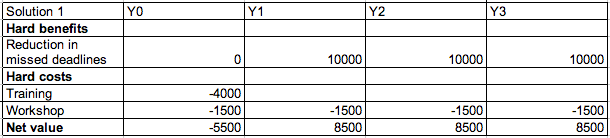
\includegraphics[scale=0.5]{Pictures/cost-benefit1.png}
    \caption{Cost benefit of Podio Work processes (units in DKK)}
\end{figure}


\subsubsection{Roll out}

\subsubsection{Training}
Forslag: Experts and normal users
\subsubsection{Data conversion}
Converting all the existing Podio data to be alligned with the new formal structure for information, knowledge and decisions...

\subsection{Implementation strategy}
The must effective way this solution can be implemented in the organization will be as a pilot project, where selected members of the organization will be trained in how to use the formal ... 



\section{Podio extension}
\subsection{Visions for change}
\label{visions_for_change}
This solution is at its a heart in interactive visualization of tasks and task dependencies across arranger teams. Tasks are communicated between arranger teams with the already present infrastructure present in Podio. The task window however, is extended with the following functionality and data:
\begin{itemize}
    \item Tasks can include subtasks. Subtasks are added to a task by pressing the "Add Subtask" button. When teams assign tasks to other teams, the receiving team may choose to define subtasks, that need to be completed before the assigned task can be completed. Subtasks can either be already existing tasks, or new tasks.
    \item Tasks include a "Done" description, in which the sender of the task may include a short description of when the task is considered to be done.
    \item Tasks are done when the receiving team presses the "Done" button under a task.
\end{itemize}
The data and functionality described above makes it possible to create a task map. The task map displays all active tasks in the system. A task is active if any of its subtasks are incomplete, or if it is itself a subtask to a task that is incomplete. Tasks are displayed graphically, with dependencies between them drawn as an directed arrow between them. Clicking a task will take the user to the task on Podio, where a detailed view of the task can be found. This solution will give arrangers an overview of deadlines, tasks associated with deadlines and dependencies between them across arranger teams, as to address problems discussed in (ref diagnostic map).


\subsection{Technology}
\label{sub:technology}
The solution uses the built in functionality of Podio to build custom Podio apps to create the needed modifications to Podio tasks. The task map is drawn on a webpage outside of the Podio domain, using the Podio REST API.

\subsubsection{IT systems and IT platform}
The solution is primarily dependent on the existing Podio platform. It is necessary that Podio maintains the possibility of defining custom apps and accessing Podio data through the REST API.

\subsubsection{User interfaces}
On Podio, the interface is built using the existing Podio app builder tools. The task map is displayed by some Web UI technology. Tasks are shown as nodes, and dependencies between them are shown as directed arrows. Task completion status is indicated graphically by color. (ref til mock up)

\subsection{Work organisation}
\label{sub:work_organisation}
Arrangers and team leaders will have to change their work-flow with creating tasks, to comply with the format described in section \ref{visions_for_change}. An introduction to using the task map must also be created. 

\subsection{Qualification needs}
\label{sub:qualification_needs}
The solution depends on arrangers and team leaders using Podio correctly. This means that arrangers and team leaders must know how to use Podio.

\subsection{Advantages and disadvantages}
\label{sec:advantages_disadvantages}
\begin{center}
    \begin{tabular}{ | p{7cm} | p{7cm} |}
    \hline
    \textbf{Advantages} & \textbf{Disadvantages}  \\ \hline
     Raises awareness of deadlines and dependencies between teams & Risk of arrangers not using the system\\ \hline
     Makes information about deadlines easier to find & Time must be invested in teaching arrangers how to and when to create tasks\\ \hline
     Integrated with a system that is already known and used by arrangers and team leaders & Solution is dependent on Podio maintaining custom app possibilities and a Web service interface \\ \hline
    \hline
    \end{tabular}
\end{center}


\subsection{Finances}
\subsection{Finances}
\begin{figure}[h!]
  \centering
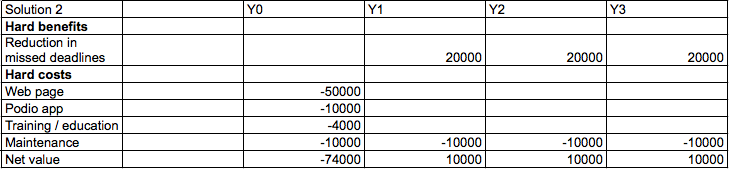
\includegraphics[scale=0.5]{Pictures/cost-benefit2.png}
    \caption{Cost benefit of Podio extension (units in DKK)}
\end{figure}

\subsection{Implementation strategy}
The solution can be implemented.




COSTS:
\begin{itemize}
    \item Development of visualisation webpage (50000 dkk)
    \item Expansion of tasks app in podio (10000 dkk)
    \item Training / education (4000 dkk)
    \item Maintenance (10000 dkk)
    \item Hosting of visualisation webpage (500 dkk)
    \item Adaption phase (time)
\end{itemize}

BENEFITS:
\begin{itemize}
    \item Avoided losses (maybe?)
    \item Better changes of making cheaper or better deals
    \item More tasks completed in time
    \item All groups know the status of the other groups' status
    \item Documentation of tasks are stored in one single place
    \item Easy to add documentation to tasks
    \item Implicitly defines when tasks are done
    \item Organisation already knows Podio
    \item Simple to use
    \item Makes it easier for the festival to innovate and improve their concepts
\end{itemize}

BULLETPOINTS:
\begin{itemize}
    \item As mentioned in the quote \ref{lol}, some offers were just obtained very shortly before
    the festival, which resulted in the price going up. The new system will make sure that offers
    are collected in time, leading to better prices. (Actual prices for the overpriced offers are
    expected to be found in the budgets.)
    \item The fact that a lot of tasks are put in different places, means that there is a chance of
    missing a deadline for a task, and thereby not making the necessary people aware of the
    existence of the task. The system will make sure that all tasks are available and visible to
    everyone.
    \item If a person leaves the organisation, the knowledge unique knowledge that the person has is
    not documented anywhere, this means that the knowledge must be gathered again, and this can be
    time consuming. Our system makes it easy to document offers and knowledge making it easy to find
    and use them in the future, thus saving time and money.
\end{itemize}

\subsection{Break even}
\label{sub:break_even}
Since the organisation only has income once a year, we think it is acceptable to invest if we break
even within in the period of two executed festivals.

\section{Implementation strategy}


